\subsection{工具链选型}\label{sec:tool-selection}

\textbf{strace 与 ftrace 机制对比}：

两者作用层次不同，开销来源也不同：

\begin{itemize}[leftmargin=2em]
  \item \textbf{strace}：通过 \texttt{ptrace} 系统调用在用户态拦截目标进程的每一次系统调用入口与出口。
        每次拦截都需要一次进程上下文切换（目标进程 $\to$ strace 进程），
        其开销与系统调用频率正相关，频繁调用时对主循环干扰极大，
        不能作为定量时序数据来源（具体扰动量级见后文实测）。

  \item \textbf{ftrace}：通过 Linux 内核 tracepoint 在内核态直接写入 ring buffer，
        \textbf{插桩本身开销极低}（纳秒级，无进程切换）。
        但将 ring buffer 内容导出至用户态文件
        （\texttt{cat /sys/kernel/debug/tracing/trace > log}
        或后台进程持续读取 \texttt{trace\_pipe}）是一次批量/持续文件 I/O，
        当 event 密集时，\textbf{导出过程本身会消耗额外 CPU 和内存带宽}，
        且实时导出期间 ring buffer 也可能覆盖旧数据（丢失事件）。
\end{itemize}

\subsubsection*{测量工具开销实测}

为定量比较各工具对主循环的扰动，本文设计了一个测量工具校准实验。
在固定 \texttt{chunk\_size=100}、目标 fps=30、episode 时长约 30 s 的同一条 \texttt{record\_loop} 上，
对比四组方案：A 组 baseline 不开任何 tracing；
B 组用 \texttt{strace -f -ttT} 包住 record 命令；
C 组开启 ftrace 仅写内核 ring buffer，episode 结束后再导出 trace；
D 组开启 ftrace 并同时启动后台进程实时读取 \texttt{trace\_pipe} 写入文件。
所有指标由 \texttt{record.py} 内部通过 \texttt{resource.getrusage()} 与 sysfs 自动采集，
写入 \texttt{analysis/timing\_stats.csv}。
表~\ref{tab:tool-overhead} 汇总了四组的核心指标，
后文分别从 FPS、上下文切换次数和阶段占比漂移三个角度逐一分析。

\begin{table}[H]
  \centering
  \caption{四组测量工具对 \texttt{record\_loop} 的扰动（每组 $n=1$，仅用于工具选型）}
  \label{tab:tool-overhead}
  \begin{tabular}{lcccc}
    \toprule
    指标 & A baseline & B strace & C ftrace 延迟 & D ftrace 实时 \\
    \midrule
    \texttt{fps\_mean}              & 16.13   & 9.53    & 13.89  & 12.48  \\
    相对 A 的 FPS 下降               & ---     & $-40.9\%$ & $-13.9\%$ & $-22.6\%$ \\
    \texttt{system\_time\_s}        & 1.40    & 2.76    & 1.37   & 1.03   \\
    \texttt{voluntary\_cs}          & 23{,}947  & 750{,}662 & 30{,}377 & 36{,}336 \\
    \texttt{involuntary\_cs}        & 78{,}436  & 541{,}334 & 84{,}481 & 52{,}907 \\
    \texttt{obs\_pct} 漂移 (pp)     & 0       & $+34.8$ & $-5.5$ & $-3.0$ \\
    \texttt{wait\_pct} 漂移 (pp)    & 0       & $-31.6$ & $-0.9$ & $-0.8$ \\
    trace 文件大小                   & ---     & 157\,MB & 168\,MB & 823\,MB \\
    \bottomrule
  \end{tabular}
\end{table}

\paragraph{FPS 下降}
图~\ref{fig:tool-fps} 给出了四组的实测 \texttt{fps\_mean} 与相对 A 组 baseline 的下降幅度。
B strace 组从 16.13 fps 跌至 9.53 fps，下降 40.9\%，
单这一项就足以排除 strace 作为正式时序数据来源的可能性。
C ftrace 延迟导出组下降 13.9\%，D ftrace 实时导出组下降 22.6\%，
两者都仍然超过设计文档定义的 $\leq 5\%$ 验收阈值；
但需要注意每组只有 1 个 episode，A 组 baseline 自身存在抖动
（如观测阶段单次冷启动时延变长会直接拉低绝对 FPS），
正式实验需补足每组 5 个 episode 后再核对方差。
即便如此，C 组优于 D 组、且两组都明显优于 B 组的相对秩序非常稳定，
能够支撑后续的工具选型。

\begin{figure}[H]
  \centering
  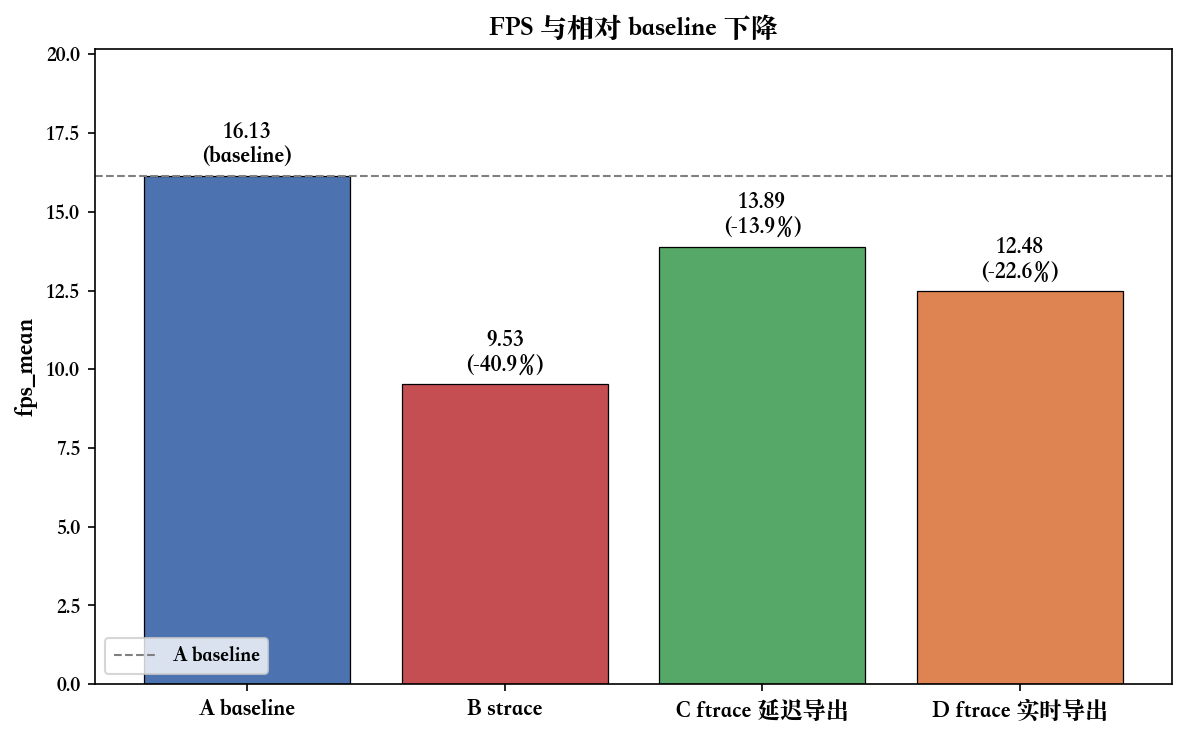
\includegraphics[width=0.85\textwidth]{../实验/04_实验环境与测量工具校准/fps_drop.png}
  \caption{四组测量工具下的 \texttt{fps\_mean} 与相对 A 组 baseline 的下降百分比}
  \label{fig:tool-fps}
\end{figure}

\paragraph{上下文切换次数}
图~\ref{fig:tool-cs} 用对数坐标对比了四组的自愿与非自愿上下文切换次数。
B strace 组的 \texttt{voluntary\_cs} 从 baseline 的约 2.4 万次飙升至约 75 万次（约 31 倍），
\texttt{involuntary\_cs} 也从 7.8 万次升至 54 万次（约 7 倍）。
这种几何级放大是 \texttt{ptrace} 机制的直接体现：
每一次系统调用都被强制中断到 strace 进程读取参数后再恢复，
因此摄像头链路中密集出现的 \texttt{pselect6}、\texttt{read}、\texttt{ioctl}
都会在切换次数上留下印记。
相比之下，C 组的切换次数仅比 baseline 高约 27\%，
D 组的额外切换主要来自后台 \texttt{cat trace\_pipe} 进程，
两者的量级都与 baseline 同档，
说明 ftrace 内核 ring buffer 插桩本身对调度路径几乎无干扰。

\begin{figure}[H]
  \centering
  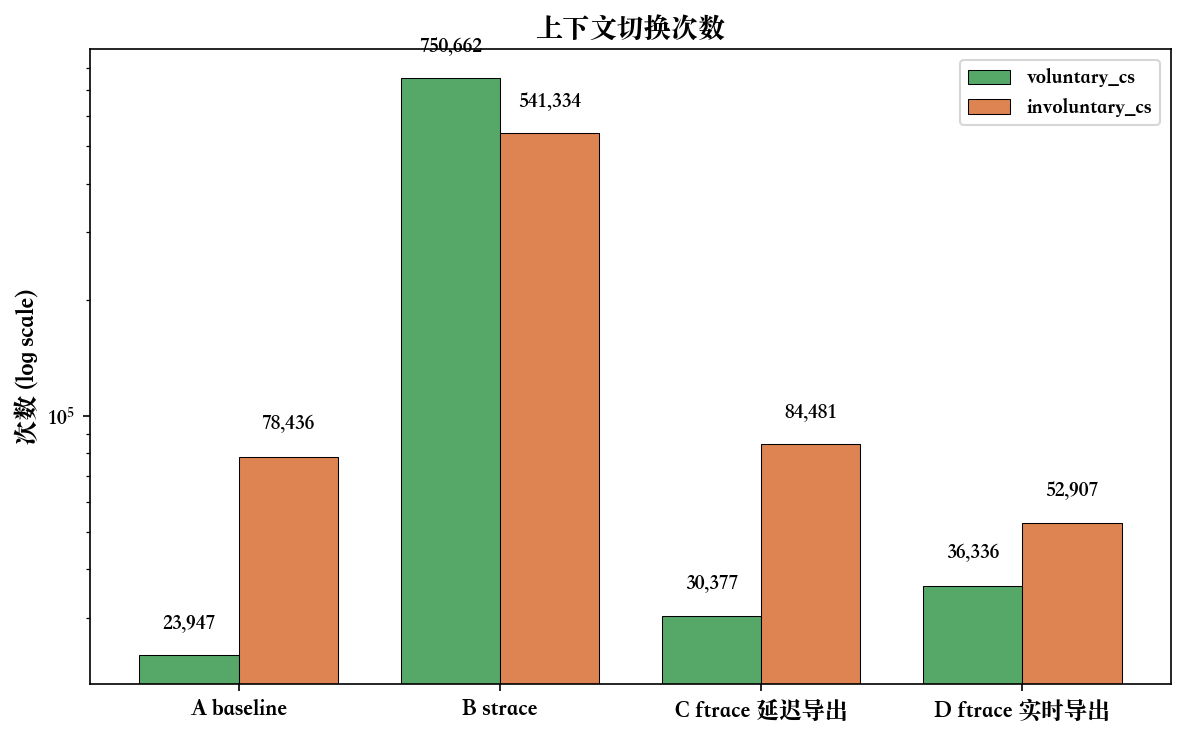
\includegraphics[width=0.85\textwidth]{../实验/04_实验环境与测量工具校准/context_switches.png}
  \caption{四组的自愿与非自愿上下文切换次数（对数坐标）}
  \label{fig:tool-cs}
\end{figure}

\paragraph{阶段占比漂移}
图~\ref{fig:tool-phase} 显示了四组各阶段占比相对 A 组 baseline 的偏移
（pp = percentage point）。
B strace 组的 \texttt{obs\_pct} 漂移高达 $+34.8$ pp，\texttt{wait\_pct} 反向漂移 $-31.6$ pp，
意味着 strace 不仅整体拉慢主循环，还\textbf{改变了阶段时间结构}：
摄像头链路中的系统调用被 \texttt{ptrace} 反复拦截，导致观测阶段被严重拉长，
\texttt{wait} 阶段反而被挤压；这种结构性扭曲使得 strace 下采集的阶段占比已经无法代表真实负载。
C 与 D 两组的所有阶段漂移都在 $\pm 8$ pp 内，
其中 wait/action 漂移均 $\leq 1$ pp，
\texttt{obs\_pct} 与 \texttt{inference\_pct} 在 $\pm 7$ pp 之间小幅互相借调，
没有出现 B 组那种数量级的结构变化；
因此可以判断 ftrace 两种方案对阶段时间结构的影响可控。

\begin{figure}[H]
  \centering
  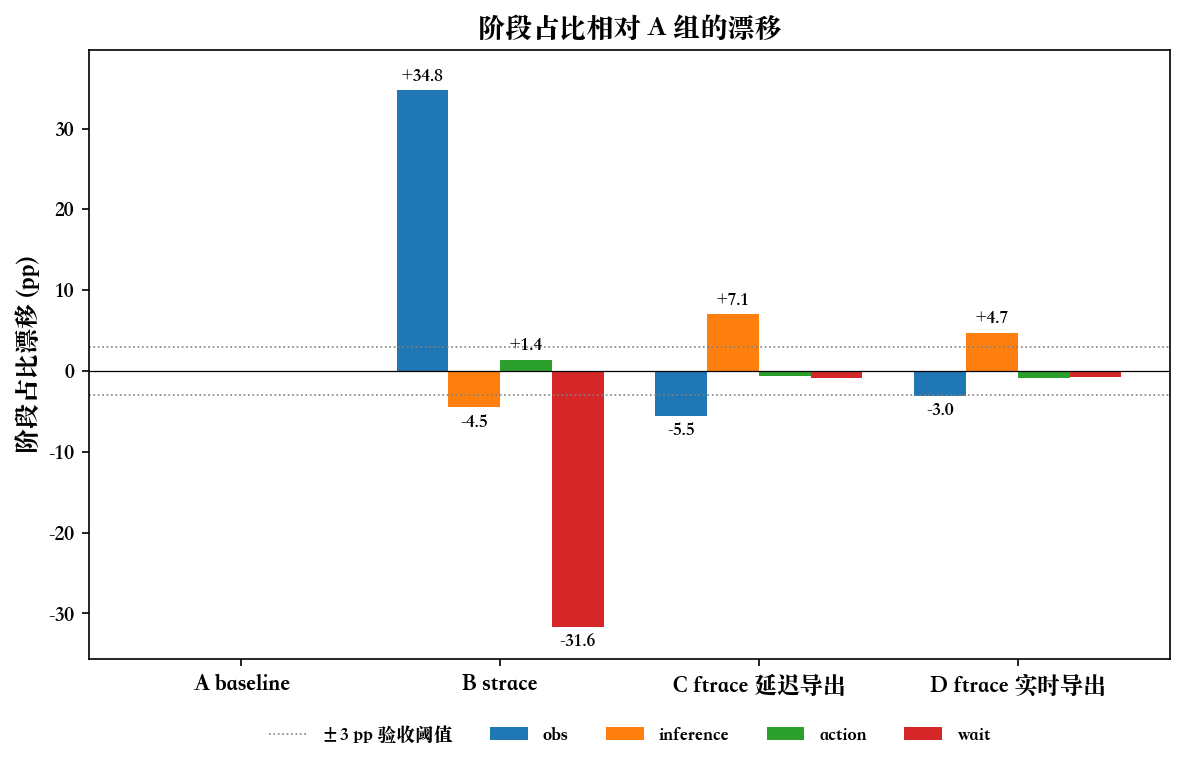
\includegraphics[width=0.85\textwidth]{../实验/04_实验环境与测量工具校准/phase_drift.png}
  \caption{四组的四阶段占比相对 A 组 baseline 的漂移（pp），灰色虚线为设计阶段提出的 $\pm 3$ pp 验收阈值}
  \label{fig:tool-phase}
\end{figure}

\paragraph{本文工具链选型}
正式实验的内核态时序数据采用 \textbf{ftrace 延迟导出}方案：
其上下文切换次数与阶段时间结构均与 baseline 同档，是单 episode 扰动最小的方案。
仅在 episode 时长延长导致 ring buffer（本文配置每 CPU 32\,MB，4 核共 128\,MB）接近溢出时，
才改用 ftrace 实时导出作为后备；其代价是 trace 数据量约为延迟导出的 4.9 倍
（823\,MB vs 168\,MB），但量级仍可承受。
strace 不参与最终定量分析，仅用于第~\ref{ch:perf} 章早期对系统调用类型分布的定性探索。

\paragraph{内核源码级插桩}

除上述标准 syscall tracepoint 外，本文还在内核源码中通过
\texttt{trace\_printk} 插入了自定义计时桩，将更精细的时间拆分信息
直接写入 ftrace ring buffer，与标准 tracepoint 事件混合输出。
标准 tracepoint 只记录系统调用入口参数和出口返回值，
无法拆分调用内部的阻塞睡眠时间与 CPU 处理时间，
也无法将文件描述符解析为设备名。

本文在两处关键路径上实现了自定义插桩：

\begin{enumerate}[leftmargin=2em]
  \item \textbf{pselect6}（\texttt{fs/select.c}，\texttt{do\_select()} 函数）：
    在函数入口通过 \texttt{ktime\_get()} 记录起始时间，
    在 \texttt{poll\_schedule\_timeout()} 前后打点计算阻塞睡眠时间，
    函数退出时输出总耗时、睡眠时间、上下文处理时间、返回值、
    就绪 fd 编号及通过 \texttt{d\_path()} 解析的设备名。
    例如，trace 中可直接观察到
    ``\texttt{fd=8, file=video0}'' 表示手眼摄像头帧就绪，
    ``\texttt{fd=9, file=video2}'' 表示固定摄像头帧就绪，
    每次等待约 30\,ms，睡眠时间约占总耗时的 99.7\%。
  \item \textbf{futex}（\texttt{kernel/futex/syscalls.c}，\texttt{do\_futex()} 函数）：
    类似地在入口和 \texttt{futex\_wait\_multiple()} 前后打点，
    输出操作码（op）、返回值、总耗时、CPU 时间和睡眠时间。
    该拆分可以直接区分 futex 快速解锁（sleep$\approx$0）与长时间等待
    （sleep 接近 total），从而判断 Python 线程间的锁竞争程度。
    实测数据显示 WAKE 操作（op=1）耗时在微秒级，
    而 WAIT 操作（op=0）的睡眠时间最高可达 1.8\,s。
\end{enumerate}

上述信息无法通过标准 tracepoint 或 kprobe 动态插桩获得：
标准 tracepoint 不提供内部时间拆分；
kprobe 回调中调用 \texttt{d\_path()} 解析 fd 路径存在死锁风险，
而 \texttt{do\_select()} 原生上下文中调用是安全的。
代价是需使用自编译内核，对本文固定的实验平台不构成额外负担。

\src{实验/04\_实验环境与测量工具校准/结论.md，内核数据搜集分析.md}
